\documentclass[12pt, cn]{elegantart}

\title{数学之美 --- The Beauty of Mathematics}
\subtitle{$\me^x=\sum_{n=0}^{\infty}\frac{x^n}{n!}=1+x+\frac{x^2}{2!}+\frac{x^3}{3!}+\frac{x^4}{4!}+\frac{x^5}{5!}+\cdots$}

\author{任\ 涛}
\email{me@tomben.me}
\date{\today}
\version{3.14}

\extrainfo{This \href{https://tomben.me/the-beauty-of-mathematics/the-beauty-of-mathematics.pdf}{booklet} was proudly made with \href{https://www.latex-project.org}{\LaTeX{}} and inspired by \href{https://github.com/ElegantLaTeX/ElegantBook}{ElegantBook}. The Chinese text is set in \href{https://source.typekit.com/source-han-serif/}{Source Han Serif}\!(思源宋体)\!\! and \href{https://docs.microsoft.com/en-us/typography/font-list/kaiti}{KaiTi}\!(\textit{楷体})\!\!. The western text is set in \href{https://www.ctan.org/pkg/newtx}{newtxtext}. And the math text is set in \href{https://www.ctan.org/pkg/newtx}{newtxmath} with a few \href{https://tex.stackexchange.com/questions/200910/replace-a-few-math-symbols-in-the-newtxmath-font}{modif{}ications}. All tools mentioned are \href{https://en.wikipedia.org/wiki/Open_source}{open source}.}

\logo{logo.pdf}
\cover{cover.jpg}


\begin{document}

\maketitle

\begin{introduction}
\item 最优性原理
\item 柯西列性质
\item 韦达定理
\item Angle of Corner
\item Property of Cauchy Series
\end{introduction}
\vspace{1cm}

\noindent 法国数学家弗朗索瓦·勒·利奥奈(Fran{\c{c}}ois Le Lionnais)说:
\begin{tcolorbox}[saying]
   Who has not been amazed to learn that the function $y = \me^x$, like a phoenix rising from its own ashes, is its own derivative?\cite{le2004} \vspace{5pt}

   有谁不被 $y = \me^x$ 惊艳过?就像浴火重生的凤凰一般,它从自身的导数中一飞冲天。
\end{tcolorbox}

\begin{center}
	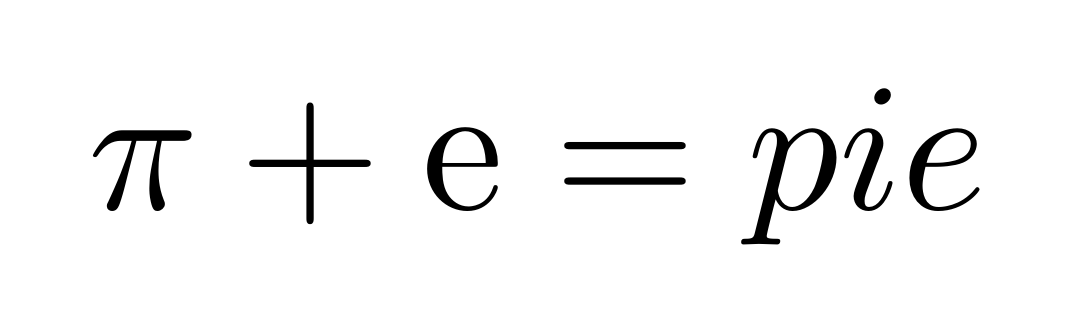
\begin{tikzpicture}
      \marmot[pie,whiskers,teeth,shadow]
      \node[anchor=east,scale=6.6,transform shape] at (-0.6,1) {$\pi + \mathrm{e}=\text{pie}$};
    \end{tikzpicture}
\end{center}

\begin{center}
	\Large\bfseries\color{structurecolor} 目\hspace{0.5em}录 \\[5pt]
	\base{structurecolor}{87}
\end{center}
\vspace{-0.8cm}
\tableofcontents
\vspace{1cm}


\section{自然数幂和公式}

\begin{theorem}{自然数平方和}{qwe}
\begin{equation}
   \sum_{i=1}^{n} i^{2}=1^2+2^2+3^2+\cdots+n^2=\frac{n(n+1)(2 n+1)}{6}
\end{equation}  
\end{theorem}

\begin{definition}{自然数平方和}{oiy}
\ding{172} 方法一:利用立方差公式累加求和

观察下面的等式:
$$\begin{array}{l}
{(n+1)^{3}-n^{3}=3 n^{2}+3 n+1}, \\ {(n)^{3}-(n-1)^{3}=3(n-1)^{2}+3(n-1)+1}, \\ {\cdots \cdots} \\ {3^{3}-2^{3}=3 \cdot 2^{2}+3 \cdot 2+1}, \\ {2^{3}-1^{3}=3 \cdot 1^{2}+3 \cdot 1+1}
\end{array}$$

将以上 $n$ 个等式相加,左边消去中间项,右边提取公因式合并,得到:
$$
(n+1)^{3}-1^{3}=3\left(1^{2}+2^{2}+\dots+n^{2}\right)+3(1+2+\dots+n)+n
$$

化简整理得到:
$$
1^{2}+2^{2}+\dots+n^{2}=\frac{n(n+1)(2 n+1)}{6}
$$

\hdashrule{\linewidth}{0.5pt}{3pt}

\ding{173} 方法二:一元函数积分法

构造二次函数:
$$f(x)=x^2,\ x \in[1, n+1]$$

将区间 $[1, n+1]$ 分割为 $n$ 个区间,则每个小曲边三角形的面积为:

$$
\int_{k}^{k+1}\left(x^{2}-k^{2}\right) \md x=\left.\frac{1}{3} x^{3}\right|_{k} ^{k+1}-\left.k^{2} x\right|_{k} ^{k+1}=k+\frac{1}{3}
$$

所以曲边三角形的面积为:
\begin{align*}
   \sum_{k=1}^{n} k^{2}&=\int_{1}^{n+1} x^{2} \md x-\sum_{k=1}^{n}\left(k+\frac{1}{3}\right)\\
   &=\left.\frac{1}{3} x^{3}\right|_{1} ^{n+1}-\sum_{k=1}^{n}\left(k+\frac{1}{3}\right)\\
   &=\frac{1}{3}(n+1)^{3}-\frac{1}{3}-\sum_{k=1}^{n} k-\sum_{k=1}^{n} \frac{1}{3}\\
   &=\frac{n(n+1)(2 n+1)}{6}
   \end{align*}
\end{definition}


\begin{theorem}{自然数立方和}{ert}
\begin{equation}
     \sum_{i=1}^{n} i^{3}=1^3+2^3+3^3+\cdots+n^3=\left(\frac{n(n+1)}{2}\right)^{2}
\end{equation}
\end{theorem}

\begin{definition}{自然数立方和}{ihj}
	观察下面的等式:
$$\begin{array}{l}
{(n+1)^{4}-n^{4}=4 n^{3}+6 n^{2}+4 n+1}, \\ {n^{4}-(n-1)^{4}=4(n-1)^{3}+6(n-1)^{2}+4(n-1)+1}, \\ {\cdots \cdots} \\ {3^{4}-2^{4}=4 \cdot 2^{3}+6 \cdot 2^{2}+4 \cdot 2+1}, \\ {2^{4}-1^{4}=4 \cdot 1^{3}+6 \cdot 1^{2}+4 \cdot 1+1}
\end{array}$$

将以上 $n$ 个等式相加,左边消去中间项,右边提取公因式合并,得到:
$$
(n+1)^{4}-1^{4}=4\left(1^{3}+2^{3}+\dots+n^{3}\right)+6\left(1^{2}+2^{2}+\dots+n^{2}\right)+4(1+2+\dots+n)+n$$

化简整理得到:
$$
1^{3}+2^{3}+\dots+n^{3}=\left(\frac{n(n+1)}{2}\right)^{2}$$
\end{definition}

\section{$\pi$ 的莱布尼茨公式}

\begin{theorem}{$\pi$ 的莱布尼茨公式}{olj}
	\begin{equation}
	\frac{\pi}{4}=1-\frac{1}{3}+\frac{1}{5}-\frac{1}{7}+\frac{1}{9}-\frac{1}{11}+\cdots %=\sum_{n=0}^{\infty} \frac{(-1)^{n}}{2 n+1}
	\end{equation}
   \vspace{-12pt}
\end{theorem}

公式 \eqref{thm:olj} 右边的展式是一个无穷级数,被称为莱布尼茨级数,这个级数收敛到 $\pi/4$。它通常也被称为格雷戈里—莱布尼茨级数,用以纪念与莱布尼茨同时代的天文学家兼数学家詹姆斯·格雷戈里。

当代有名的数论大家塞尔贝格\footnote{塞尔贝格,挪威裔美国籍数学家。由于他所做的关于黎曼 \textzeta 函数零点分布问题的出色成果,以及对素数定理的初等证明,于 1960 年荣获 Fields 奖,时年 33 岁。他还于 1986 年荣获 Wolf 数学奖。}(Atle Selberg)

\begin{tcolorbox}[saying]
	我喜欢数学的一个动机就是公式 \eqref{thm:olj}。这个公式实在美极了,单数 $1,3,5\cdots$这样的组合可以给出 $\pi$。对于一个数学家来说,此公式正如一幅美丽图画或风景。
\end{tcolorbox}

\begin{conclusion}
回归分析(regression analysis)是确定两种或两种以上变量间相互依赖的定量关系的一种统计分析方法。运用十分广泛,回归分析按照涉及的变量的多少,分为一元回归和多元回归分析;按照因变量的多少,可分为简单回归分析和多重回归分析;按照自变量和因变量之间的关系类型,可分为线性回归分析和非线性回归分析。
\end{conclusion}

\begin{solution}
即 $D(x)$ 在 $[0,1]$ 上是 Lebesgue 可积的并且积分值为零。但 $D(x)$ 在 $[0,1]$ 上不是 Riemann 可积的。
\end{solution}

\begin{remark}
Overleaf 上,中文需要使用 \lstinline{XeLaTeX} 进行编译,英文可以使用 \lstinline{PDFLaTeX} 与 \lstinline{XeLaTeX}。
\end{remark}


\section{巴塞尔问题}

\begin{theorem}{巴塞尔问题}{Basel}
	\begin{equation}
		\sum_{n=1}^{\infty} \frac{1}{n^{2}}=\frac{1}{1^{2}}+\frac{1}{2^{2}}+\frac{1}{3^{2}}+\cdots=\frac{\pi^2}{6}
	\end{equation}
\end{theorem}

\section{欧拉公式}

\begin{theorem}{欧拉公式}{euler}
	\begin{equation}
		\mathrm{e}^{\mi \pi}+1=0
	\end{equation}
   \begin{equation}
      \me^{\mi x}=\cos x+\mi \sin x
   \end{equation}
   \vspace{-15pt}
\end{theorem}

\section{拉马努金恒等式}

\begin{theorem}{拉马努金恒等式}{lmu}
	\begin{equation}
		3=\sqrt{1+2 \sqrt{1+3 \sqrt{1+4 \sqrt{1+5 \sqrt{1+\cdots}}}}}
	\end{equation}
\end{theorem}

斯里尼瓦瑟·拉马努金(Srinivasa Ramanujan)

\begin{remark}
	2013 年 11 月 4 日,\href{https://www.weibo.com/1894798092/Ah8QTrRae}{广州恒大微博}
\end{remark}

\section{连分数}
\begin{theorem}{连分数}{lfr}
	\begin{equation}
	0.618=\frac{1}{1+\frac{1}{1+\frac{1}{1+\cdots}}}
	\end{equation}

	\begin{equation}
	\pi=3+\frac{1}{7+\frac{1}{15+\frac{1}{1+\frac{1}{292+\frac{1}{1+\frac{1}{1+\ddots}}}}}}
	\end{equation}
\end{theorem}

\section{欧拉常数}

\begin{theorem}{欧拉常数}{euc}
\begin{equation}
		\gamma=\lim _{n \rightarrow \infty}\left( 1+\frac{1}{2}+\frac{1}{3}+\cdots+\frac{1}{n} -\ln n\right)=0.57721566490\cdots
\end{equation}
\end{theorem}


%%%%%%%%%%%%%%%%%%%%%%%%%%%%%%%%%%%%%%%%%%%%%%%%%%%%%%%%%%
\begin{proposition}{Gauss Equation}{lup}
\begin{align*}
\iint\limits_{\Sigma}P(x,y,z)\mathrm{d}y{\rm{d}}z+Q(x,y,z){\rm{d}}z{\rm{d}}x+R(x,y,z){\rm{d}}x{\rm{d}}y=\iiint\limits_\Omega\left(\frac{\partial{Q}}{\partial{x}}+\frac{\partial{P}}{\partial{y}}+\frac{\partial{R}}{\partial{z}}\right){\rm{d}}{x}{\rm{d}}{y}{\rm{d}}{z}
\end{align*}
\end{proposition}


\begin{property}\label{property:cauchy}
柯西列的性质
\begin{enumerate}
\item $\{x_k\}$ 是柯西列,则其子列 $\{x_k^i\}$ 也是柯西列。
\item $x_k\in \mathcal{R}^n$,$\rho(x,y)$ 是欧几里得空间,则柯西列收敛,$(\mathcal{R}^n,\rho)$ 空间是完备的。
\end{enumerate}
\end{property}

我们将通过三个步骤定义可测函数的积分。首先定义非负简单函数的积分。以下设 $E$ 是 $\mathcal{R}^n$ 中的可测集。

\begin{equation}
   \label{inter2}
   \int_0^1 D(x)\md x = \int_0^1 \chi_{Q_0} (x) \md x = m(Q_0) = 0
\end{equation}
即 $D(x)$ 在 $[0,1]$ 上是 Lebesgue 可积的并且积分值为零。但 $D(x)$ 在 $[0,1]$ 上不是 Riemann 可积的。

\begin{note}
在本模板中,引理(lemma),推论(corollary)的样式和定理的样式一致,包括颜色,仅仅只有计数器的设置不一样。
\end{note}

\begin{property}\label{property:cauchy}
柯西列的性质
\begin{enumerate}
\item $\{x_k\}$ 是柯西列,则其子列 $\{x_k^i\}$ 也是柯西列。
\item $x_k\in \mathcal{R}^n$,$\rho(x,y)$ 是欧几里得空间,则柯西列收敛,$(\mathcal{R}^n,\rho)$ 空间是完备的。
\end{enumerate}
\end{property}

\begin{proposition}{$y = \me^x$}{fki}
Who has not been amazed to learn that the function $y = \me^x$, like a phoenix rising from its own ashes, is its own derivative? --- Francois Le Lionnais

有谁不被 $y = \me^x$ 惊艳过? 就像浴火重生的凤凰一般,它从自身的导数中一飞冲天 --- 弗朗西斯 $\cdot$ 勒利奥内
\end{proposition}


\nocite{*}
\bibliography{reference}
\addcontentsline{toc}{section}{\S \;\;\, 参考资料}

\clearpage
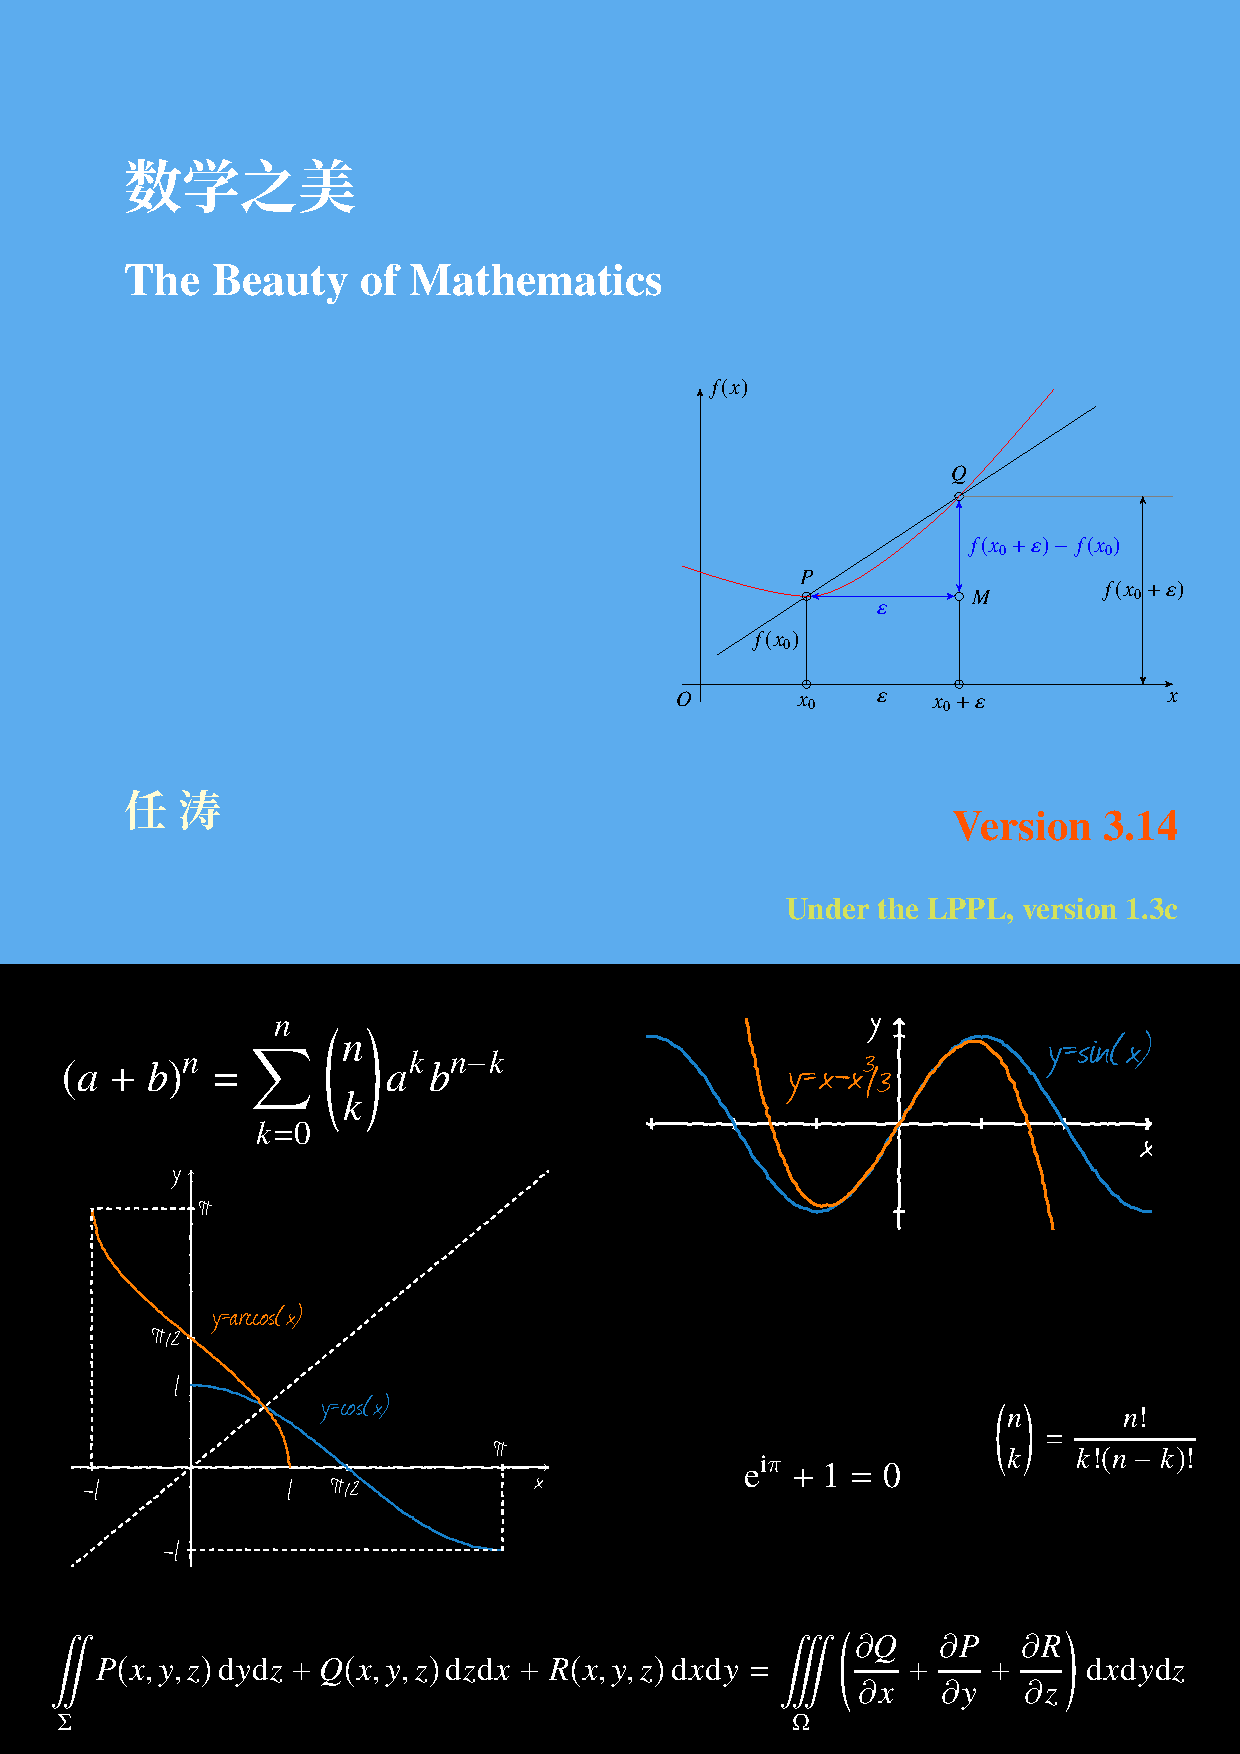
\includepdf{./endpage/endpage.pdf}

\end{document}